\documentclass[12pt]{article}

\usepackage{amsmath}
\usepackage{amssymb}
\usepackage{enumitem}
\usepackage{geometry}
\geometry{margin=1in}

\usepackage{tikz}
\usetikzlibrary{
    arrows.meta,
    calc,
    angles,
    quotes,
    decorations.pathmorphing
}
\usepackage[american]{circuitikz}


\setlist[enumerate,1]{label=\arabic*.}

\begin{document}

\begin{center}
\Large \textbf{Ultra-Hard Physics Paper}
\end{center}

\begin{enumerate}

%=========================================================
%=========================================================
\item \textbf{Rotational Dynamics + Non-Inertial Effects} 

A uniform solid disk of mass $M$ and radius $R$ is mounted on a frictionless vertical axle. A small rough block of mass $m$ is gently placed at the rim. The coefficient of static friction between the block and disk is $\mu$. A constant torque $\tau$ is applied about the axis causing angular acceleration.

Assume the block does not slip initially and the normal reaction adjusts instantaneously. Taking into account both tangential and radial pseudo forces in the rotating frame, determine the maximum angular acceleration for which pure rolling without slipping is maintained.

Maximum angular acceleration is:

\begin{center}
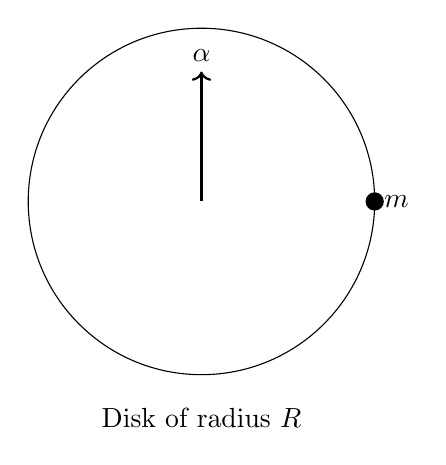
\begin{tikzpicture}[scale=1.1]
\draw (0,0) circle (2);
\fill (2,0) circle (3pt);
\node[right] at (2,0) {$m$};
\draw[->,thick] (0,0) -- (0,1.5);
\node[above] at (0,1.5) {$\alpha$};
\node at (0,-2.5) {Disk of radius $R$};
\end{tikzpicture}
\end{center}

A) $ \dfrac{\mu mg}{R\left(\frac{M}{2}+m\right)} $

B) $ \dfrac{\mu g}{R}\left(\dfrac{m}{\frac{M}{2}+m}\right) $

C) $ \dfrac{\mu g}{R} $

D) $ \dfrac{\mu mg}{R(M+m)} $
%=========================================================
%=========================================================
\item \textbf{Rotation + Electromagnetic Coupling}

A light cylindrical shell of mass $M$ and radius $R$ is free to rotate about its axis. A light string is wound around it carrying a particle of mass $m$ and charge $q$. The system is placed in a uniform vertical electric field $E$ directed upward.

The string does not slip and rotational inertia must be included. Assuming downward direction positive and neglecting air resistance, determine the linear acceleration of the particle immediately after release.

Acceleration is:

\begin{center}
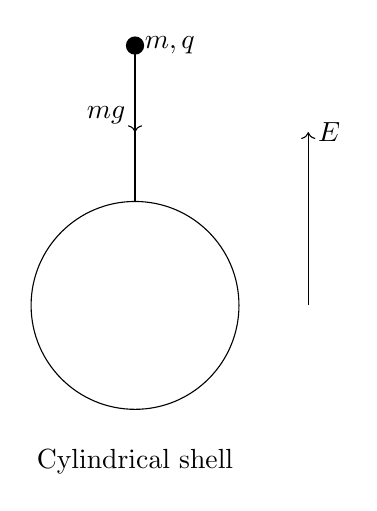
\begin{tikzpicture}[scale=1.1]
\draw (0,0) circle (1.2);
\draw (0,1.2) -- (0,3);
\fill (0,3) circle (3pt);
\node[right] at (0,3) {$m,q$};
\draw[->] (2,0) -- (2,2);
\node[right] at (2,2) {$E$};
\draw[->] (0,3) -- (0,2);
\node[left] at (0,2.2) {$mg$};
\node at (0,-1.8) {Cylindrical shell};
\end{tikzpicture}
\end{center}

A) $ \dfrac{mg-qE}{m+M} $

B) $ \dfrac{mg+qE}{m+M} $

C) $ \dfrac{mg-qE}{m} $

D) $ \dfrac{mg-qE}{m+\frac{M}{2}} $
%=========================================================
%=========================================================
\item \textbf{Thermodynamics + Small Oscillation Equilibrium Shift} 

An ideal gas is enclosed in a vertical cylinder fitted with a frictionless piston of mass $M$. The piston is connected to a vertical spring of constant $k$. Initially the system is in equilibrium at volume $V_0$ under gravity $g$. Suddenly the effective gravitational acceleration increases to $2g$.

Assuming the process remains isothermal and the displacement from equilibrium is small enough to linearize pressure variation, determine the fractional change in equilibrium volume.

\begin{center}
\begin{tikzpicture}[scale=1.1]
\draw (0,0) rectangle (3,4);
\draw (0,4) rectangle (3,4.5);
\draw[decorate,decoration={zigzag,segment length=4}] (1.5,4.5) -- (1.5,6);
\node at (1.5,3) {Gas};
\node[right] at (3,4.25) {Piston $M$};
\node[right] at (1.6,5.3) {$k$};
\end{tikzpicture}
\end{center}

A) $ \dfrac{Mg}{kV_0} $

B) $ 2\dfrac{Mg}{kV_0} $

C) $ -\dfrac{Mg}{kV_0} $

D) zero

%=========================================================
%=========================================================
\item \textbf{Charged Particle Dynamics with Combined Fields} 

A particle of charge $q$ and mass $m$ moves in a plane perpendicular to a uniform magnetic field $B$. In addition, a weak radial electric field $E(r)=\alpha r$ exists directed outward.

Assuming circular motion of radius $R$ and treating the electric field as a small perturbation, determine the modified angular frequency to first order in $\alpha$.

\begin{center}
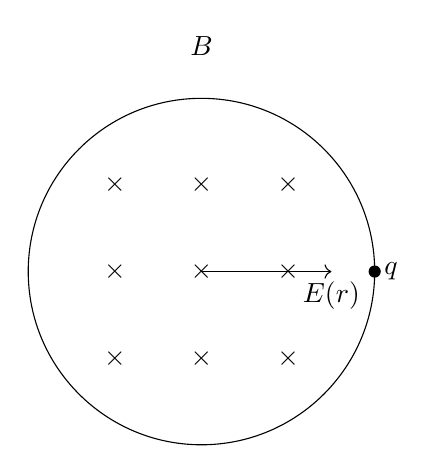
\begin{tikzpicture}[scale=1.1]
\draw (0,0) circle (2);
\fill (2,0) circle (2pt);
\node[right] at (2,0) {$q$};

\draw[->] (0,0) -- (1.5,0);
\node[below] at (1.5,0) {$E(r)$};

% Magnetic field into page
\foreach \x in {-1,0,1}
  \foreach \y in {-1,0,1}
    \node at (\x,\y) {$\times$};

\node at (0,2.6) {$B$};
\end{tikzpicture}
\end{center}

A) $ \dfrac{qB}{m} $

B) $ \dfrac{qB}{m}+\dfrac{\alpha}{B} $

C) $ \dfrac{qB}{m}-\dfrac{\alpha}{B} $

D) $ \dfrac{qB}{m}+\dfrac{\alpha R}{B} $

%=========================================================
\item \textbf{Stability of Rotating System} 

A light rigid horizontal rod of length $L$ has identical masses $m$ suspended from its ends by light vertical strings of length $h$. The system rotates with constant angular velocity $\omega$ about a vertical axis through the center of the rod.

As angular velocity increases, the masses begin to tilt outward. Using equilibrium in rotating frame and considering small angle approximation, determine the critical angular speed at which vertical configuration becomes unstable.



\begin{center}
\begin{tikzpicture}[scale=1.1]
\draw (-2,0) -- (2,0);
\draw[dashed] (-2,0) -- (-2,-2);
\draw[dashed] (2,0) -- (2,-2);
\draw (-2,0) -- (-2.5,-2);
\draw (2,0) -- (2.5,-2);
\fill (-2.5,-2) circle (3pt);
\fill (2.5,-2) circle (3pt);
\node[left] at (-2.5,-2) {$m$};
\node[right] at (2.5,-2) {$m$};
\draw[->] (0,0) -- (0,1.5);
\node[above] at (0,1.5) {$\omega$};
\end{tikzpicture}
\end{center}

A) $ \sqrt{\dfrac{g}{h}} $

B) $ \sqrt{\dfrac{Mg}{mh}} $

C) $ \sqrt{\dfrac{(M+2m)g}{mh}} $

D) $ \sqrt{\dfrac{mg}{Mh}} $

%=========================================================
\item \textbf{Electromagnetic Induction with Time-Varying Field} 

A conducting rod slides down smooth inclined rails of angle $\theta$ forming a closed circuit of resistance $R$. The magnetic field perpendicular to the plane varies as $B=B_0(1+\beta t)$.

Ignoring self-inductance but accounting for motional and transformer emf simultaneously, determine how terminal velocity depends on $\beta$.



\begin{center}
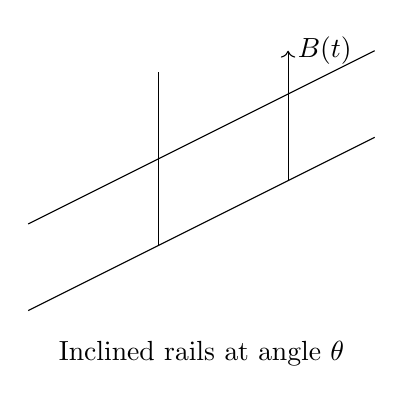
\begin{tikzpicture}[scale=1.1]
\draw (0,0) -- (4,2);
\draw (0,1) -- (4,3);
\draw (1.5,0.75) -- (1.5,2.75);
\draw[->] (3,1.5) -- (3,3);
\node[right] at (3,3) {$B(t)$};
\node at (2,-0.5) {Inclined rails at angle $\theta$};
\end{tikzpicture}
\end{center}

A) independent of $\beta$

B) decreases with $\beta$

C) increases with $\beta$

D) becomes zero

%=========================================================
\item \textbf{Perturbation of Potential Minimum}

A particle moves in one dimension under potential
\[
U(x)=\alpha x^4-\beta x^2+\gamma x
\]
where $\gamma$ is very small compared to other parameters.

Using perturbative expansion about symmetric equilibrium, determine proportional dependence of shift in equilibrium position to first order in $\gamma$.

A) $ \dfrac{\gamma}{\beta} $

B) $ \dfrac{\gamma}{\alpha} $

C) $ \dfrac{\gamma}{\beta^2} $

D) $ \dfrac{\alpha}{\gamma} $

%=========================================================
\item \textbf{Orbital Decay with Dissipation}

A satellite of mass $m$ moves in a nearly circular orbit of radius $R$ around Earth. It experiences a small drag force proportional to instantaneous velocity $F=-kv$.

Assuming decay is slow so orbit remains nearly circular at each instant, use energy balance to determine proportional dependence of $\dfrac{dR}{dt}$ on radius.

A) $R$

B) $\dfrac{1}{R}$

C) $\dfrac{1}{R^2}$

D) constant

%=========================================================
\item \textbf{Electrostatics + Work-Energy}

A parallel plate capacitor connected to an ideal battery has its plate separation slowly increased by an external agent while charge redistributes continuously.

Taking into account work done by battery and change in field energy, determine mechanical work done by the external agent.

A) equal to increase in electrostatic energy

B) twice increase

C) half increase

D) zero

%=========================================================
\item \textbf{Central Force Motion}

A projectile is fired vertically from Earth surface with speed $u$. Gravitational acceleration varies with distance as $g(r)=GM/r^2$.

Using conservation of mechanical energy without approximation, determine relation satisfied by maximum radial distance attained.

A) $ \dfrac{1}{r_{\max}}=\dfrac{1}{R}-\dfrac{u^2}{2GM} $

B) $ \dfrac{1}{r_{\max}}=\dfrac{1}{R}+\dfrac{u^2}{2GM} $

C) $ r_{\max}=R+\dfrac{u^2}{2g} $

D) independent of $GM$

%=========================================================
\item \textbf{Impulse + Oscillation with Dissipation}

Two identical blocks connected by light spring lie on rough horizontal surface with small coefficient of friction $\mu$. An impulse $J$ is applied instantaneously to one block.

Assuming motion remains small amplitude and friction acts as perturbation, determine leading dependence of reduction in maximum compression of spring.

A) $\mu J$

B) $\mu J^2$

C) $\mu^2$

D) independent of $\mu$

%=========================================================
\item \textbf{Rotational EMF}

A circular conducting loop rotates with constant angular speed about a diameter in uniform magnetic field.

Taking into account time variation of flux through instantaneous plane of loop, determine time dependence of induced emf.

A) $\sin\omega t$

B) $\cos\omega t$

C) constant

D) zero

%=========================================================
\item \textbf{Atomic Physics Scaling}

An electron is in circular Bohr orbit with total energy $E$. Nuclear charge is slowly increased to twice its value so motion remains adiabatic.

Determine new total energy in terms of original energy.

A) $4E$

B) $\dfrac{E}{4}$

C) $2E$

D) $\dfrac{E}{2}$

%=========================================================
\item \textbf{Anharmonic Oscillator}

A particle oscillates in potential
\[
U(x)=\alpha x^6+\beta x^2
\]
with small amplitude $A$.

Using expansion of restoring force and energy method, determine leading correction to oscillation frequency due to anharmonic term.

A) $\alpha A^4$

B) $\alpha A^2$

C) $\beta A^2$

D) independent of $A$

%=========================================================
\item \textbf{Loop-the-Loop Energy}

A small body slides without friction inside a vertical circular track of radius $R$. It is given just enough speed at bottom to maintain contact throughout the loop.

Using condition of zero normal reaction at highest point and energy conservation, determine difference in mechanical energy between lowest and highest points.



\begin{center}
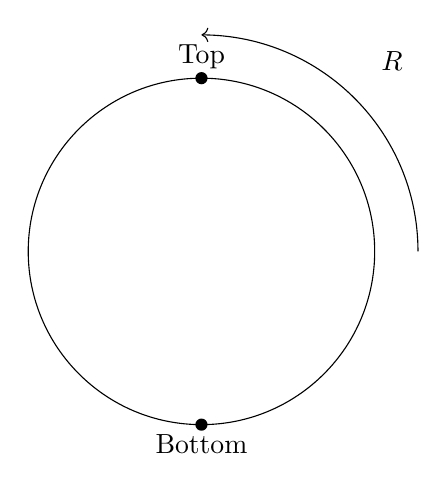
\begin{tikzpicture}[scale=1.1]
\draw (0,0) circle (2);
\fill (0,-2) circle (2pt);
\node[below] at (0,-2) {Bottom};
\fill (0,2) circle (2pt);
\node[above] at (0,2) {Top};
\draw[->] (2.5,0) arc (0:90:2.5);
\node at (2.2,2.2) {$R$};
\end{tikzpicture}
\end{center}


A) $2mgR$

B) $3mgR$

C) $\dfrac{5}{2}mgR$

D) $\dfrac{3}{2}mgR$

%=========================================================

\end{enumerate}

\end{document}